\documentclass[12pt]{article}

\usepackage{amsmath}
\usepackage{amssymb}
\usepackage{calc}
\usepackage{units}
\usepackage{graphicx}
\usepackage[pdftex]{hyperref}
\usepackage{subfig}
\usepackage[margin=1in]{geometry}
\usepackage{listings}
\usepackage[numbers,sort&compress]{natbib}
\usepackage{bm}
\usepackage{paralist}
\usepackage[draft]{fixme}
\usepackage{textcomp}
\usepackage{yorkdefs}

\hypersetup{
  breaklinks=true,
  pdftitle={Refraction and Dispersion},
  pdfauthor={Kevin R. Lynch},
  pdfsubject={Phyiscs, Electricity and magnetism, Optics},
  pdfkeywords={reflection},
  pdflang={en-US},
}

\title{Reflection}
\author{}
%Kevin R. Lynch
%\date{2012-04-26}
\date{}

\begin{document}

\maketitle

\section{Objectives}
\label{sec:objectives}

\begin{enumerate}
\item To understand reflection in optical systems, and
\item To determine quantitatively the parameters of various curved
  mirrors. 
\end{enumerate}

\section{Introduction}
\label{sec:introduction}

\fixme{Need a good introduction}

\section{Theory}
\label{sec:theory}

\begin{figure}
  \centering
%% No rights to use this if we stop using Serway and Jewett ... don't
%% publish on the publicly accessible web!
  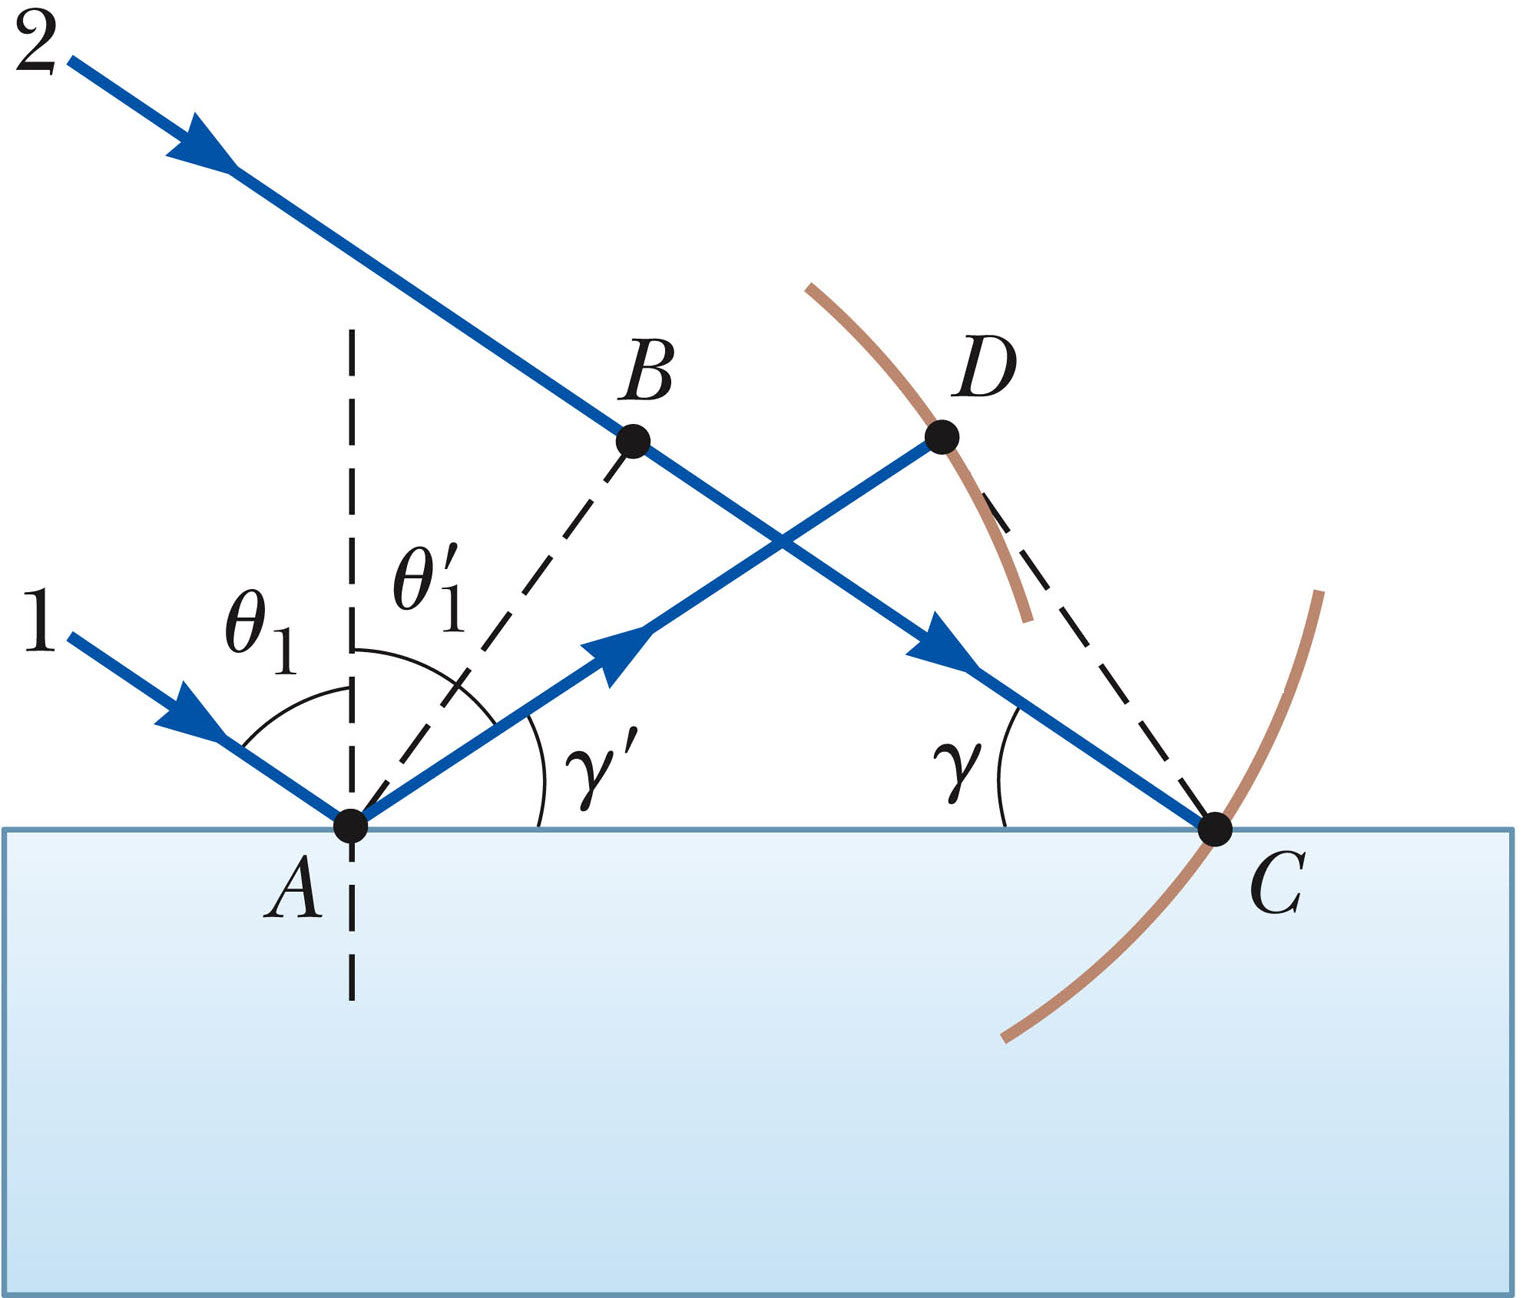
\includegraphics[width=\textwidth/2]{figures/3519}  
  \caption{The Incident and reflected rays discussed in the text.}
  \label{fig:defs}
\end{figure}

In this lab, we will work in the limit of ray optics - that is, where
the feature size of objects we illuminate is much larger than the
wavelength of the light.  In this limit, we can treat the interfaces
between different materials as perfectly smooth surfaces.  At those
surfaces, light changes direction, or \textit{reflects} from the
surface.  The relationship between the angle of the incident ray and
the angle of the reflected ray can be predicted using \textit{Huygen's
  Princple}:\footnote{Serway and Jewett, \textit{Physics for
    Scientists and Engineers}, 8th Ed.}
\begin{quote}
  All points on a given wave front are taken as point soures for the
  production of spherical secondary waves - wavelets - that propagate
  outward.  After some time interval has passes, the new position of
  the wave front is the surface tangent to the wavelets.
\end{quote}
Figure~\ref{fig:defs} shows rays incident on a surface, along with a
wavefront.  In the figure, rays 1 and 2 are parallel, and propagate to
points $A$ and $B$, arriving at the same time (the definition of a
wavefront).  In the time interval $\delta t$, ray 1 reflects from the
surface and propagates to point $D$, while ray 2 reaches point $C$ in
the same interval.  Since both rays travel in the same material during
$\delta t$, they must travel the same distance: $AD = BC$.
Now\footnote{And this is the key point, one which the Serway and
  Jewett text inexplicably leaves out!} at the point of reflection,
each ray will generate a spherical wavelet; at any later time, those
expanding wavelets will, by symmetry, construct a wavefront that is
normal to the direction of propagation.  Since the wavefront passed
through $AB$ at the earlier time, it must pass through $CD$ at the
later instant, so the wavefront must be perpendicular to the ray $AD$!
Geometrically, then, the two triangles $DAC$ and $BCA$ are congruent,
and $\gamma = \gamma'$.  Therefore the incident and reflected angles
must be equal:
\begin{gather*}
  \theta_I = \theta_R\ .
\end{gather*}
This type of reflection from an ideal, smooth surface is called
\textit{specular} reflection, as opposed to the \textit{diffuse}
reflection off a rough surface.

\begin{figure}
  \centering
%% No rights to use this if we stop using Serway and Jewett ... don't
%% publish on the publicly accessible web!
  \subfloat[][A Concave Mirror]{
    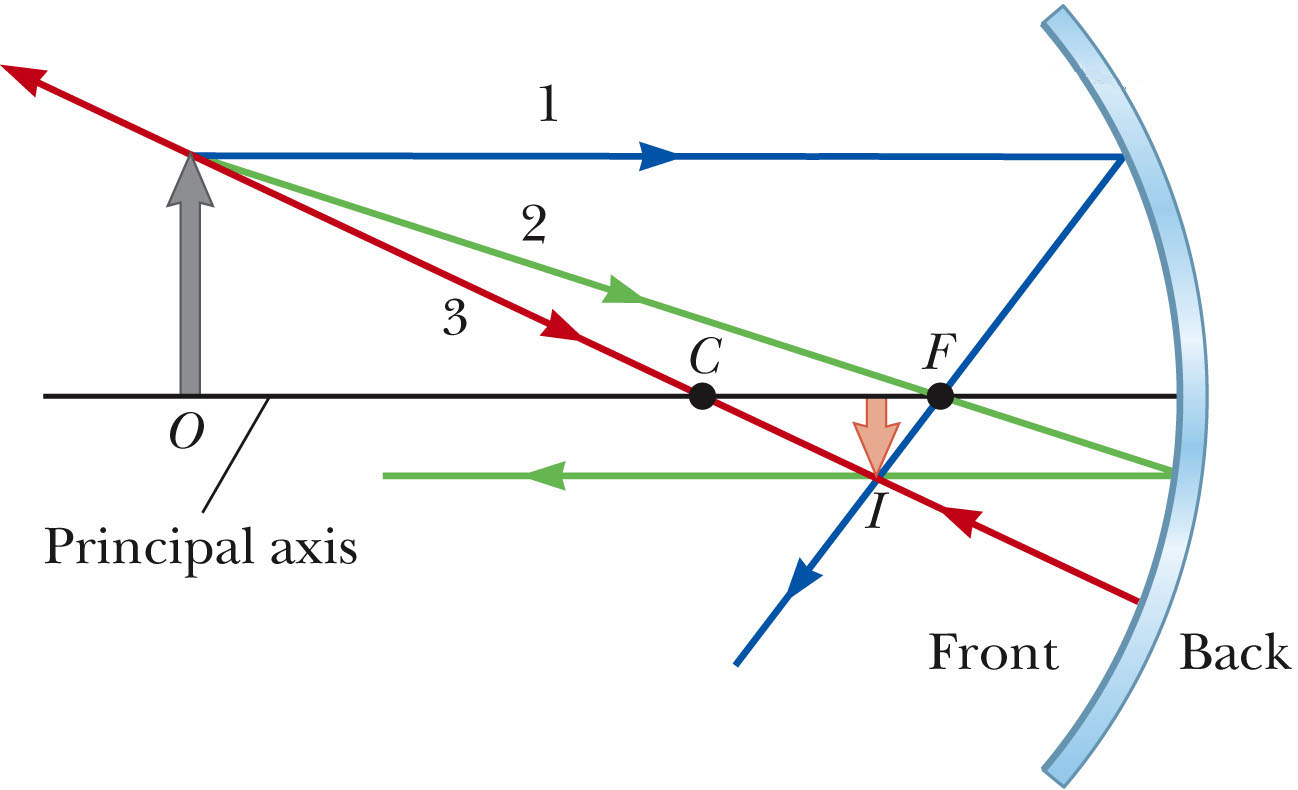
\includegraphics[width=\textwidth/2-0.1in]{figures/3613a}
  }
%% No rights to use this if we stop using Serway and Jewett ... don't
%% publish on the publicly accessible web!
  \subfloat[][A Convex Mirror]{
    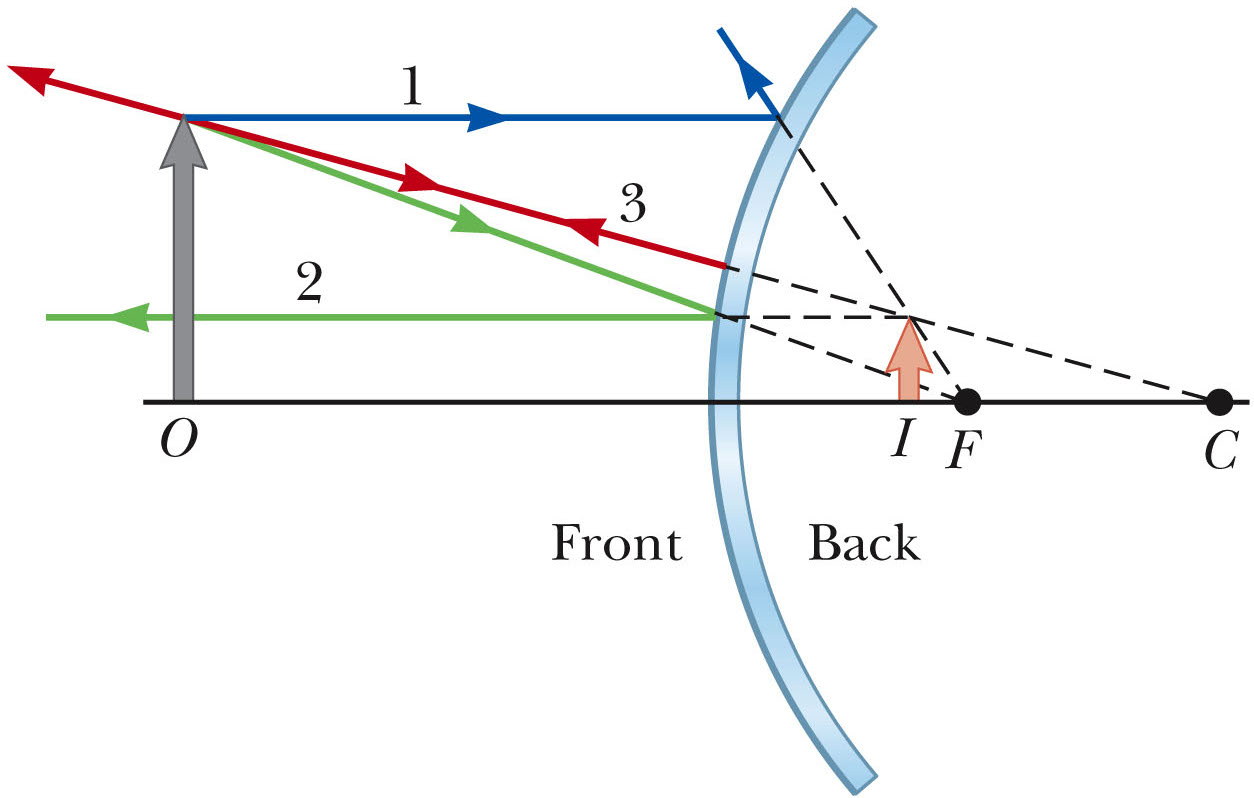
\includegraphics[width=\textwidth/2-0.1in]{figures/3613c}
  }
  \caption{These figures illustrate the ray diagram construction for
    determining the image position and magnification, as described in
    the text.}
  \label{fig:mirrors}
\end{figure}
If we curve the mirrors, the seemingly simple relation gives rise to a
rich set of phenomena, which have a close relationship to the behavior
of thin lenses.  Just like lenses, mirrors can be used to focus images
of objects, and those images will be scaled copies of the objects; see
Figure~\ref{fig:mirrors}.  We focus here on the behavior of mirrors
that are circular or spherical sections; other types of mirrors
(parabolic, hyperbolic, etc) exist, but they have significantly more
complicated properties than what we will discuss here.

Describing the behavior of spherical mirrors quantitatively requires a
few definitions.  First, define the \textit{principal axis} as a ray
that runs through the center of curvature (the center of the circle
that the mirror lies on) and the center of the circular mirror
section.  Next, put the base of the object on the principal ray.
Define the distance along the principal ray from the object to the
mirror as $p$, and the distance from the image to the mirror as $q$..
The object and image may be either \textit{real} - if rays actually
travel the distance to the mirror - or \textit{virtual} - if the rays
do not actually travel the distance to the mirror.  These distances
are related to the curvature of the mirror by
\begin{gather*}
  \frac{1}{p} + \frac{1}{q} = \frac{1}{f}\ .
\end{gather*}
The focal length, $f$, of the mirror is simply half the radius of
curvature $r$ of the mirror
\begin{gather*}
  f = \frac{r}{2}\ .
\end{gather*}
When the object or image are real, the distance is taken (by
convention) as positive; if virtual, the distance is taken as
negative.  You can prove that the focal length of a concave mirror is
positive, while the focal length of a convex mirror is negative.

The image and object distances also give the image magnification,
which is the ratio of the image height $h_i$ to the object height
$h_o$:
\begin{gather*}
  M  = \frac{h_i}{h_o} = -\frac{q}{p}\ ,
\end{gather*}
where a negative magnification corresponds to an image
\textit{inverted} with respect to the object orientation.

We can graphically illustrate the properties of a curved mirror by
constructing \textit{ray diagrams}.  For a concave mirror, draw three
rays from the top of the object (the base, of course, lies on the
principal axis):
\begin{enumerate}
\item Ray 1, parallel to the principal axis to an intersection with
  the mirror.  The reflected ray will pass through the focal point.
\item Ray 2, through the focal point.  The reflected ray will be
  parallel to the principal axis.
\item Ray 3, through the center of curvature.  Since this is normal to
  the surface (it's along a radius) this will be reflected back on
  itself.
\end{enumerate}
The intersection point of these three rays (real or virtual) defines
the image.  For a convex mirror, since the focus and center of
curvature lie on the \textit{other} side of the mirror from the
object, the construction varies slightly; determine the modifications
by reference to Figure~\ref{fig:mirrors}.  To find the focal point, we
utilize a set of rays all parallel to the principal axis; this is
equivalent to having an object at infinity, and the image then appears
with zero height \textit{at} the focal point.

\section{Procedures}
\label{sec:procedures}

You should receive a laser pointer, a set of flat and curved mirrors,
sheets of white paper, rulers and protractors.  

\subsection{Flat Mirrors}
\label{sec:flat}

Using your flat mirror, perform ray tracing for a number of incident
angles (say, 5).  Measure the reflected angles to confirm or refute
the equality of $\theta_I$ and $\theta_R$.  What is your largest
source of uncertainty?

\subsection{Curved Mirrors}
\label{sec:curved}

\begin{figure}
  \centering
  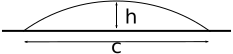
\includegraphics[width=\textwidth/2]{figures/chord}
  \caption{The radius of curvature of a circular segment can be
    determined if the chord length, $c$, and the height, $h$, of the
    segment are known.}
  \label{fig:chord}
\end{figure}
For both the concave and convex mirrors, determine the focal lengths by
the parallel ray construction method, and compare this to the focal
length determined from the radius of curvature.  Assuming the mirror
is a segment of a circle, you can determine the radius of curvature
$r$ by measuring the chord $c$ and the height $h$ of the segment:
\begin{gather*}
  r = \frac{h^2 + (c/2)^2}{2h}\ ;
\end{gather*}
the variables are defined in Figure~\ref{fig:chord}.  The radius is
positive for concave mirror, and negative for a convex mirror.

Now that you have determined the focal length, use your lasers to
recreate the image construction outlined in Figure~\ref{fig:mirrors}.
There are three cases you should consider: for the convex mirror, find
the location and size of the virtual image; for the concave mirror,
determine the location and size of the images for objects that are
closer to and further from the mirror than the focal point.  For all
three cases, measure $p$ and $q$, as well as the transverse heights of
the objects and images.

\newpage
 
\section*{Pre-Lab Exercises}

Answer these questions as instructed on Blackboard; make sure to
submit them before your lab session!

\begin{enumerate}
\item The focal length of a convex lens is negative.  What does this
  tell you about the size of the magnification of the image?  The
  sign? 
\item For a concave lens, an object is place three focal lengths from
  the mirror.  Where is the image?  What is its orientation?
\item Does a flat mirror produce a real or virtual image?  What is its
  magnification? 
\end{enumerate}

\newpage

\section*{Post-Lab Exercises}

\begin{enumerate}
\item Does your data from Section~\ref{sec:flat} support the Huygen's
  Construction where $\theta_I = \theta_R$?  Discuss your
  uncertainties.
\item From your data in Section~\ref{sec:curved}, what are the focal
  lengths and radii of curvature for your two mirrors?  Discuss your
  uncertaintites.  Are the mirrors circular?  How do you know?
\item From your data in Section~\ref{sec:curved}, do the predicted
  magnifications match the measured magnifications?  Discuss your
  uncertainties. 
\item Discuss briefly whether you have met the objectives of the lab
  exercises.
\end{enumerate}

\end{document}

%%% Local Variables: 
%%% mode: latex
%%% TeX-master: t
%%% End: 
